To fully understand how residential consumers adjust their consumption behavior in response to price changes under the TOU program, it is necessary to explicitly examine the relationship between the size of the price changes and the change in each of the two distinct categories of household electricity consumption for each of the three periods (i.e., the pre-peak, peak, and post-peak periods). In other words, quantifying the impact of the marginal price change on residential electricity consumption will help evaluate the role of the intraday price variation under TOU electricity pricing. In the analysis, I utilize the magnitude of the price changes, from the flat rate, in the peak rate period for all three periods. There are two reasons why I exploit the price increases in the peak rate period rather than those in the corresponding period. One reason is that in the pre- and post-peak periods, the estimated changes in household electricity consumption do not show any apparent correlation with the price decreases in the corresponding periods.\footnote{As discussed in the previous section, the price increases in the peak rate period clearly drive the changes in the two types of electricity consumption in the same period.} The other reason is that the price changes in the peak rate period well encapsulate two different price incentives under TOU pricing in off-peak hours, price incentives for load-shedding and load-shifting.\footnote{Before and after the peak period, the two price incentives are proportional to the magnitude of the price increases in the peak period.} Using the following econometric model, I quantitatively determine the relationship:
\begin{align}
\small
\begin{split}
    kWh_{ith} \ 
    & = \ \beta_{1} HDD_{t} \ + \ \beta_{2} HDD_{t}^{*} \\
    & \hspace{0.7cm} + \ \left( \beta_{3} \ + \ \beta_{4} HDD_{t} \ + \ \beta_{5} HDD_{t}^{*} \right) \mathds{1}[\text{Treatment}]_{i} \\
    & \hspace{0.7cm} + \ \left( \beta_{6} \ + \ \beta_{7} HDD_{t} \ + \ \beta_{8} HDD_{t}^{*} \right) \mathds{1}[\text{Treatment}]_{i} \Delta PC_{i} \\
    & \hspace{0.7cm} + \ \left( \beta_{9} \ + \ \beta_{10} HDD_{t} \ + \ \beta_{11} HDD_{t}^{*} \right) \mathds{1}[\text{Post}]_{t} \\
    & \hspace{0.7cm} + \ \left( \beta_{12} \ + \ \beta_{13} HDD_{t} \ + \ \beta_{14} HDD_{t}^{*} \right) \mathds{1}[\text{Treatment \& Post}]_{it} \\
    & \hspace{0.7cm} + \ \left( \beta_{15} \ + \ \beta_{16} HDD_{t} \ + \ \beta_{17} HDD_{t}^{*} \right) \mathds{1}[\text{Treatment \& Post}]_{i} \Delta PC_{i} \ + \ \kappa_{dw} \ + \ \epsilon_{ith}
\end{split}
\label{Eq:Model-Specification_Breakdown-of-Hourly-Average-Treatment-Effect-as-a-Linear-Function-of-Price-Changes}
\end{align}

The model is the same with (\ref{Eq:Model-Specification_Breakdown-of-Hourly-Average-Treatment-Effect}) except for interaction terms between treatment-status-relevant indicator variables (i.e., $\mathds{1}[\text{Treatment}]_{i}$ and $\mathds{1}[\text{Treatment \& Post}]_{it}$) and $\Delta PC_{i}$, where $\Delta PC_{i}$ is the difference between the peak-hour prices in the treatment period and the flat rate in the baseline period. The coefficients of the second interaction term (i.e., $\beta_{15}$, $\beta_{16}$, and $\beta_{17}$) capture the impacts of deploying TOU tariffs on household electricity consumption as a linear function of the degree of a peak-demand-hour price change. 

\afterpage{
    \begin{table}[t!]
        \centering
        \caption{Hourly Treatment Effects as a Linear Function of Peak-Rate-Period Price Changes}
        \label{Table:Hourly-ATEs-as-a-Linear-Function-of-Peak-Rate-Period-Price-Changes_Coefficients-of-Interest-only}
        \vspace{0.3cm}
        \small
        \begin{adjustbox}{scale = 1.0}
            \begin{threeparttable}
                \begin{tabular}{@{\extracolsep{40pt}}lccc}
                    \\[-5.5ex]
                    \hline \hline
                    \\[-3.0ex]
%                    & \multicolumn{15}{c}{Dependent Variable} \\
%                    \\[-3.0ex]
%                    \cline{2-100}
%                    \\[-3.0ex]
                    & \multicolumn{3}{c}{Hourly Electricity Consumption  (kWh/Hour)} \\
                    \\[-3.0ex]
                    & (1) & (2) & (3) \\
                    \\[-3.0ex]
                    \hline
                    \\[-2.0ex]
                    $\mathbb{1}$[Treatment \& Post] & $-$0.045 & $-$0.028 & $-$0.053 \\
                    & (0.029) & (0.035) & (0.035) \\
                    & & & \\
                    $\mathbb{1}$[Treatment \& Post] $\times$ $\Delta$PC & 0.002 & $-$0.005$^{**}$ & 0.002 \\
                    & (0.002) & (0.002) & (0.002) \\
                    & & & \\
                    $\mathbb{1}$[Treatment \& Post] $\times$ HDDs & $-$0.0001 & $-$0.010$^{**}$ & $-$0.001 \\
                    & (0.004) & (0.004) & (0.004) \\
                    & & & \\
                    $\mathbb{1}$[Treatment \& Post] $\times$ HDDs$^{*}$ & 0.001 & 0.012$^{**}$ & 0.005 \\
                    & (0.005) & (0.006) & (0.005) \\
                    & & & \\
                    $\mathbb{1}$[Treatment \& Post] $\times$ HDDs $\times$ $\Delta$PC & 0.00001 & 0.0002 & $-$0.0001 \\
                    & (0.0002) & (0.0002) & (0.0003) \\
                    & & & \\
                    $\mathbb{1}$[Treatment \& Post] $\times$ HDDs$^{*}$ $\times$ $\Delta$PC & $-$0.0002 & $-$0.0003 & 0.00004 \\
                    & (0.0003) & (0.0003) & (0.0003) \\
                    & & & \\
                    \hline
                    \\[-2.0ex]
                    Description of Period & Pre-Peak & Peak & Post-Peak \\
                    Period of Hours & 15 to 16 & 17 to 18 & 19 to 20 \\
                    Knot & 10 & 10 & 10 \\
                    FEs: Day of Week by Half-Hourly Time Window & Yes & Yes & Yes \\
                    Observations & 1,006,200 & 1,006,200 & 1,006,200 \\
                    Adjusted R$^{2}$ & 0.024 & 0.047 & 0.040 \\
                    \\[-2.0ex]
                    \hline \hline
                    \\[-4.5ex]
                \end{tabular}
                \begin{tablenotes}[flushleft]
                    \footnotesize
                    \item \textit{Note}: * $p < 0.1$, ** $p < 0.05$, and *** $p < 0.01$.
                \end{tablenotes}
            \end{threeparttable}
        \end{adjustbox}
    \end{table}
}

The estimates of the six coefficients of interest (i.e., from $\beta_{12}$ to $\beta_{17}$) presented in Table \ref{Table:Hourly-ATEs-as-a-Linear-Function-of-Peak-Rate-Period-Price-Changes_Coefficients-of-Interest-only} are summarized graphically in Figure \ref{Figure:Treatment-Effects-as-a-Linear-Function-of-Price-Changes-in-the-Peak-Rate-Period}, which is extensively exploited throughout this paper. And this figure, showing the estimated treatment effects for the two consumption channels and the sum of the treatment effects in each of the three intervals, re-confirms the finding of peak-rate-period price increases' diminishing returns in \cite{Peaking-Interest:How-Awareness-Drives-the-Effectiveness-of-Time-of-Use-Electricity-Pricing_Prest_2020}. 
\afterpage{
    \begin{figure}[t!]
        \centering
        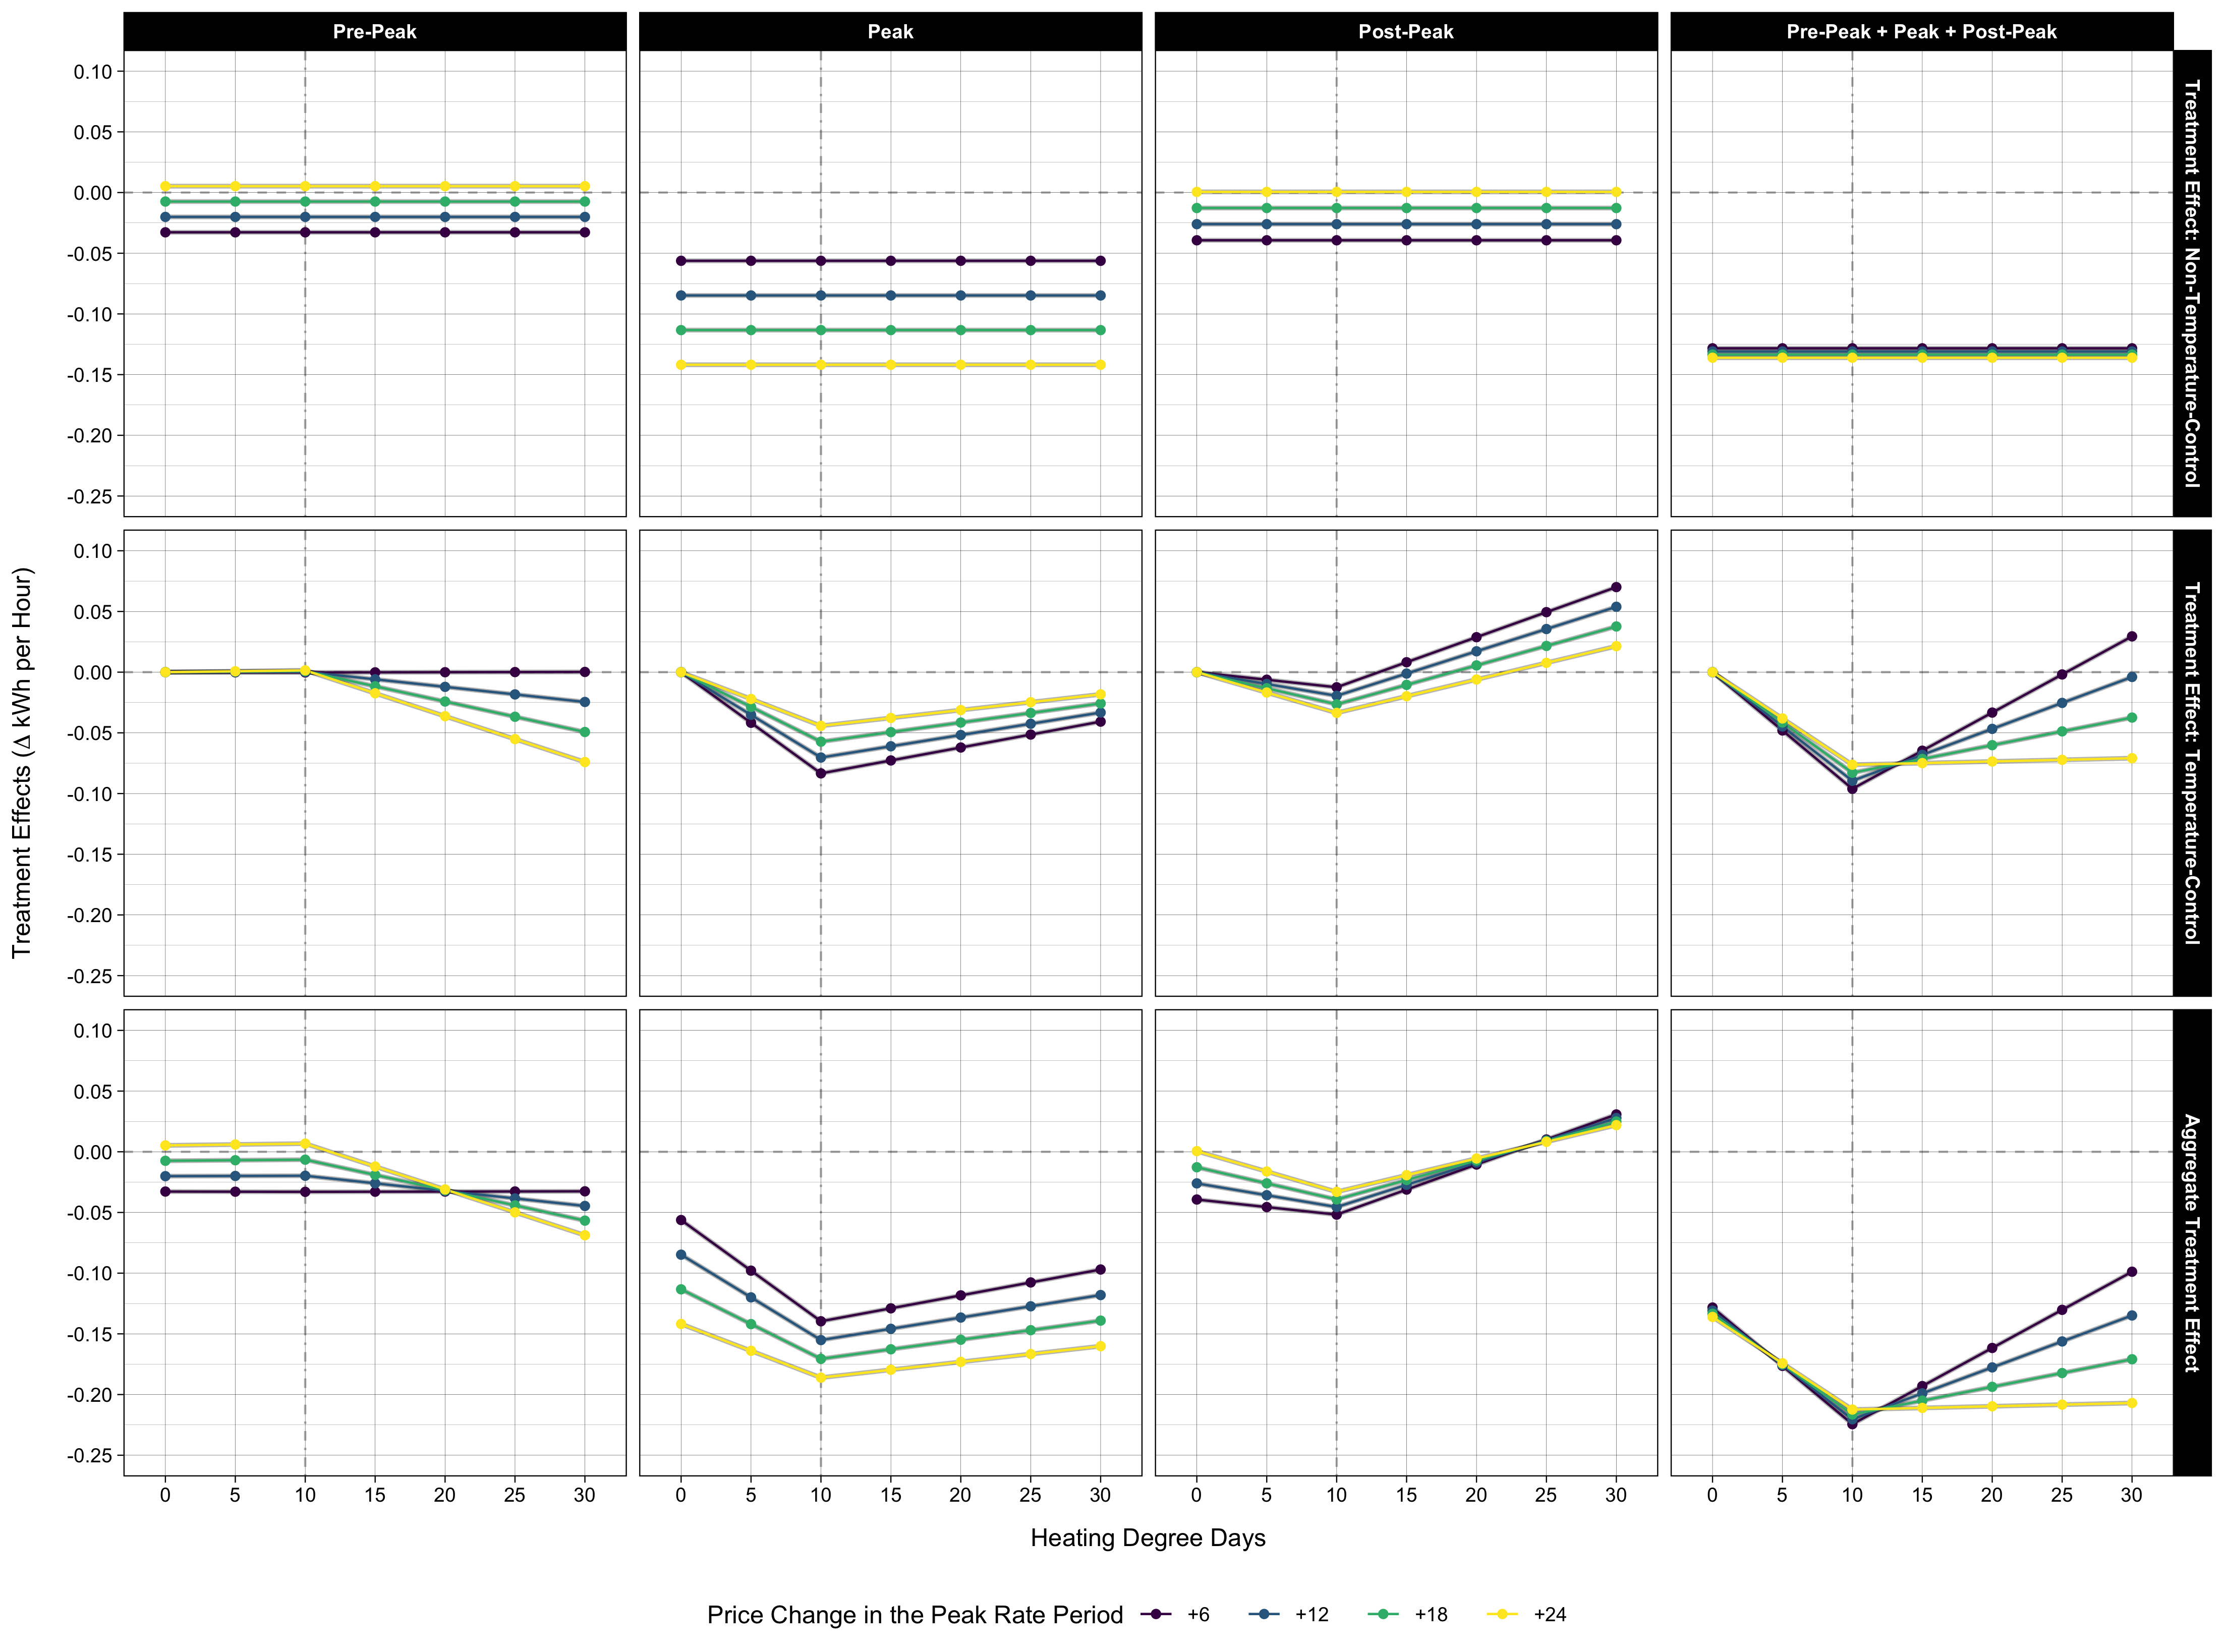
\includegraphics[scale = 0.10]{03_Chapter-2/00A_Figures/Figure_Predicted-Electricity-Savings_By-Intervals-and-HDDs_Spline_Knot-10.png}
        \caption{Treatment Effects as a Linear Function of Peak-hour Price Changes}
        \caption*{
            {\small
            \textit{Note}: This figure depicts, for four different price changes in the peak rate period, estimated treatment effects as a linear function of price changes. The first row in the figure shows the treatment effects on non-temperature-control-driven household electricity consumption. The treatment effects on temperature-control-related residential electricity consumption are illustrated in the second row. The aggregate effects are presented in the last row. The first three columns correspond to the three two-hour periods (i.e., pre-peak, peak, and post-peak periods). The fourth column demonstrates the total changes in the three periods. 
        }}
        \label{Figure:Treatment-Effects-as-a-Linear-Function-of-Price-Changes-in-the-Peak-Rate-Period}
    \end{figure}
} 

In the peak rate period, the reduction in non-temperature-control-associated electricity consumption increased as the magnitude of a peak-hour price increase grew (see the panel in the first row of the second column of Figure \ref{Figure:Treatment-Effects-as-a-Linear-Function-of-Price-Changes-in-the-Peak-Rate-Period}). On the contrary, at given daily HDDs, the reduction in temperature-control-related electricity consumption weakly moved towards zero as the size of a peak-demand-hour tariff escalation increased (see the panel in the second row of the second column of Figure \ref{Figure:Treatment-Effects-as-a-Linear-Function-of-Price-Changes-in-the-Peak-Rate-Period}). As well illustrated in the panel in the third row of the second column of Figure \ref{Figure:Treatment-Effects-as-a-Linear-Function-of-Price-Changes-in-the-Peak-Rate-Period}, for a given value of daily HDDs, the differences in treatment effect across the level of price growth are seemingly dampened when the estimated treatment effects from two distinct categories of electricity consumption are aggregated due to the opposite response to peak-hour price increases in the two consumption categories.\footnote{The last row of Figure \ref{Figure:Treatment-Effects-as-a-Linear-Function-of-Price-Changes-in-the-Peak-Rate-Period} shows the sum of the first and second rows.} Indeed, this empirical result is consistent with the finding discussed in the paper that a higher price results in a larger diminution in electricity demand, while additional gains diminish in the peak interval. 

In the two-hour interval before the peak rate period, the two types of residential electricity consumption continue to respond differently to the peak price for given daily HDDs, but the pattern is now switched. The pre-peak period exhibits a more significant reduction in non-temperature-control-driven electricity consumption for a more minor change in peak-hour price (see the panel in the first row of the first column of Figure \ref{Figure:Treatment-Effects-as-a-Linear-Function-of-Price-Changes-in-the-Peak-Rate-Period}). By contrast, the larger the magnitude of a peak-rate-period price change, the wider the diminution in temperature-control-related electricity consumption during the pre-peak period (see the panel in the second row of the first column of Figure \ref{Figure:Treatment-Effects-as-a-Linear-Function-of-Price-Changes-in-the-Peak-Rate-Period}). For the same reason as in the peak period, the aggregate treatment effects of the TOU tariffs described in the last row of the first column of Figure \ref{Figure:Treatment-Effects-as-a-Linear-Function-of-Price-Changes-in-the-Peak-Rate-Period} are seemingly less sensitive to peak-hour prices. Note that regarding electricity consumption for heating during the pre-peak period, TOU electricity pricing played a role only when household heating needs were sufficiently high. 

Irish residential consumers adjusted their electricity consumption behavior during the post-peak period as well. As in the pre-peak period, consumption changes stemming from non-temperature-control-related electricity use increased as the size of a peak-demand-hour rate change diminished (see the panel in the first row of the third column of Figure \ref{Figure:Treatment-Effects-as-a-Linear-Function-of-Price-Changes-in-the-Peak-Rate-Period}). The TOU-price-induced change in temperature-control-driven electricity consumption evolved over daily HDDs somewhat complicatedly. Though depending on the magnitude of a peak-hour price increase, TOU tariffs reduced household electricity consumption for heating on Ireland's typical winter days in that period. Interestingly, the CER TOU program provoked additional heating-related consumption during the post-peak period on extremely cold days in Ireland. In addition, as the level of peak-demand-hour price alteration grew, the profile of measured treatment effect for temperature-control-associated consumption moved downward. Consequently, a higher price increase in the peak rate period resulted in a more significant reduction in electricity consumption for heating when heating demands were lower, while a smaller addition to electricity consumption for heating on cold winter days (see the panel in the second row of the third column of Figure \ref{Figure:Treatment-Effects-as-a-Linear-Function-of-Price-Changes-in-the-Peak-Rate-Period}). Altogether, as shown in the last row of the third column of Figure \ref{Figure:Treatment-Effects-as-a-Linear-Function-of-Price-Changes-in-the-Peak-Rate-Period}, the aggregate treatment effects of the TOU program in the post-peak period are superficially moderated because of households' opposite responses to peak-demand-hour price increases in the two distinct channels of electricity consumption.  

In summary, under TOU electricity pricing, the degree of a price change in peak-demand hours, not just its existence, still matters to residential consumers' electricity consumption. The empirical results above suggest that the opposite directional changes in the two channels of electricity consumption make Irish households appear insensitive to the time-varying price structure. In other words, their high sensitivity to TOU prices is revealed only when their electricity consumption is disaggregated. Together with the empirical findings in previous sections, the results imply that three simultaneously interacting factors govern the dynamics of residential electricity consumption under TOU pricing: the timing when electricity is consumed, daily HDDs, and the magnitude of price increase in the peak rate period.  
